\documentclass[letterpaper,11pt]{article}
\oddsidemargin -1.0cm \textwidth 17.5cm

\usepackage[utf8]{inputenc}
\usepackage[activeacute,spanish, es-lcroman]{babel}
\decimalpoint
\usepackage{amsfonts,setspace}
\usepackage{amsmath}
\usepackage{amssymb, amsmath, amsthm}
\usepackage{comment}
\usepackage{float}
\usepackage{amssymb}
\usepackage{dsfont}
\usepackage{anysize}
\usepackage{multicol}
\usepackage{enumerate}
\usepackage{graphicx}
\usepackage[left=1.5cm,top=2cm,right=1.5cm, bottom=1.7cm]{geometry}
\setlength\headheight{1.5em} 
\usepackage{fancyhdr}
\usepackage{multicol}
\usepackage{hyperref}
\usepackage{wrapfig}
\usepackage{subcaption}
\usepackage{siunitx}
\usepackage{cancel}
\usepackage{mdwlist}
\usepackage{svg}
\pagestyle{fancy}
\fancyhf{}
\renewcommand{\labelenumi}{\normalsize\bfseries P\arabic{enumi}.}
\renewcommand{\labelenumii}{\normalsize\bfseries (\alph{enumii})}
\renewcommand{\labelenumiii}{\normalsize\bfseries \roman{enumiii})}


\begin{document}

\fancyhead[L]{\itshape{Facultad de Ciencias F\'isicas y Matem\'aticas}}
\fancyhead[R]{\itshape{Universidad de Chile}}

\begin{minipage}{11.5cm}
    \begin{flushleft}
        \hspace*{-0.6cm}\textbf{FI1000-1 Introducción a la Física Clásica}\\
        \hspace*{-0.6cm}\textbf{Profesor:} Ignacio Bordeu\\
        \hspace*{-0.6cm}\textbf{Auxiliares:} Alejandro Cartes \& Simón Yáñez\\
        \hspace*{-0.6cm}\textbf{Ayudante:} Javier Cubillos\\
    \end{flushleft}
\end{minipage}

\begin{picture}(2,3)
    \put(366, 10){
\includegraphics[scale=0.9]{2020-1/Imágenes/logo/dfi-fcfm.pdf}}
\end{picture}

\begin{center}
	\LARGE\textbf{Trabajo Dirigido \#3}\\
	\Large{Preparación C2}
\end{center}

\vspace{-1cm}
\begin{enumerate}\setlength{\itemsep}{0.4cm}

\rfoot[]{pág. \thepage}

\item[]

% ---------------------------------------------------------
% ando sin inspiración :( no encontré más ejercicios buenos 
% 
% se repite el msje
% ---------------------------------------------------------

\item Los bloques A y B están sobre dos planos inclinados, unidos mediante una cuerda ideal que pasa através de una polea. El coeficiente de rozamiento estático del bloque A con el plano de la izquierda es despreciable y el del bloque B con el plano de la derecha es $\mu_e$. La masa del bloque B corresponde a $m_b$. Determine el rango de masas del bloque A ($m_a$) para el cual el sistema se encuentra en equilibrio estático.

\begin{figure}[htbp]
  \centering
  \svgpath{../../2023-1/img/TD 3}
  \includesvg[width=0.55\linewidth]{P1 - TD 3.svg}
\end{figure}




\item Un disco está rotando a velocidad angular constante $\vec{\Omega}$.  Sobre este disco se encuentra un pequeño disco de hockey con masa $m$, ubicado a una distancia $R$ del centro. El disco de hockey está conectado a otro bloque con masa $M$, que cuelga debajo a través de una cuerda ideal que pasa por un orificio sin fricción en el centro del disco. El coeficiente de fricción estática entre el disco y el plato es $\mu_s$. Determine el rango de valores de $M$ para que el bloque no suba ni baje.

\begin{figure}[htbp]
  \centering
  \svgpath{../../2023-1/img/TD 3}
  \includesvg[width=0.65\linewidth]{P2 - TD 3.svg}
\end{figure}

\begin{multicols}{2}
\item Un aro de radio $R$ dispuesto en forma vertical se mueve horizontalmente como se indica en la figura. En el punto $O$ se fija el extremo de un resorte de constante elástica $k$ y de largo natural $\ell_0 = \pi R /2$. En el otro extremo del resorte se adhiere una argolla de masa $m$. El resorte envuelve el aro de modo que su forma es siempre la de un arco de círculo de radio $R$. A consecuencia del movimiento del aro, el resorte mantiene una elongación constante caracterizada por un arco de ángulo $\theta$ con respecto al eje del aro. Determine la aceleración del aro.

\columnbreak

\begin{figure}[H]
    \centering
    \svgpath{../../2021-2/img/aux6}
    \includesvg[width=0.8\linewidth]{aro.svg}     
\end{figure}

\end{multicols}

\item Un bloque de masa $M$ comienza a deslizar, desde una altura $H$, por una cuña de ángulo característico $\alpha$. Si el coeficiente de roce es $\mu_c$, determine el trabajo realizado por la fuerza de roce y el peso.

\begin{figure}[H]
    \centering
    \svgpath{../../2021-2/img/aux7}
    \includesvg[width=0.25\linewidth]{p1.svg}
\end{figure}

\item Un bloque de masa $m$ se deja caer por un plano sin roce inclinado en un ángulo $\theta$. Cuando el bloque alcanza el final del plano, se desliza sobre una cinta que se mueve con rapidez $v_b$. Sea $\mu_k$ y $\mu_s$ los coeficientes de roce cinético y dinámico, respectivamente, de la cinta

\begin{enumerate}
    \item Determine el trabajo realizado por el peso
    
    \item Utilizando la parte anterior, determine la rapidez del bloque al llegar al final del plano
    
    \item Determine la distancia $d$ que recorre el bloque a lo largo de la cinta para que alcance la misma rapidez de esta.
    
    ¿Qué pasa si la rapidez calculada en la parte (b) es menor? ¿mayor? Separe ambas situaciones
\end{enumerate}

\begin{figure}[H]
    \centering
    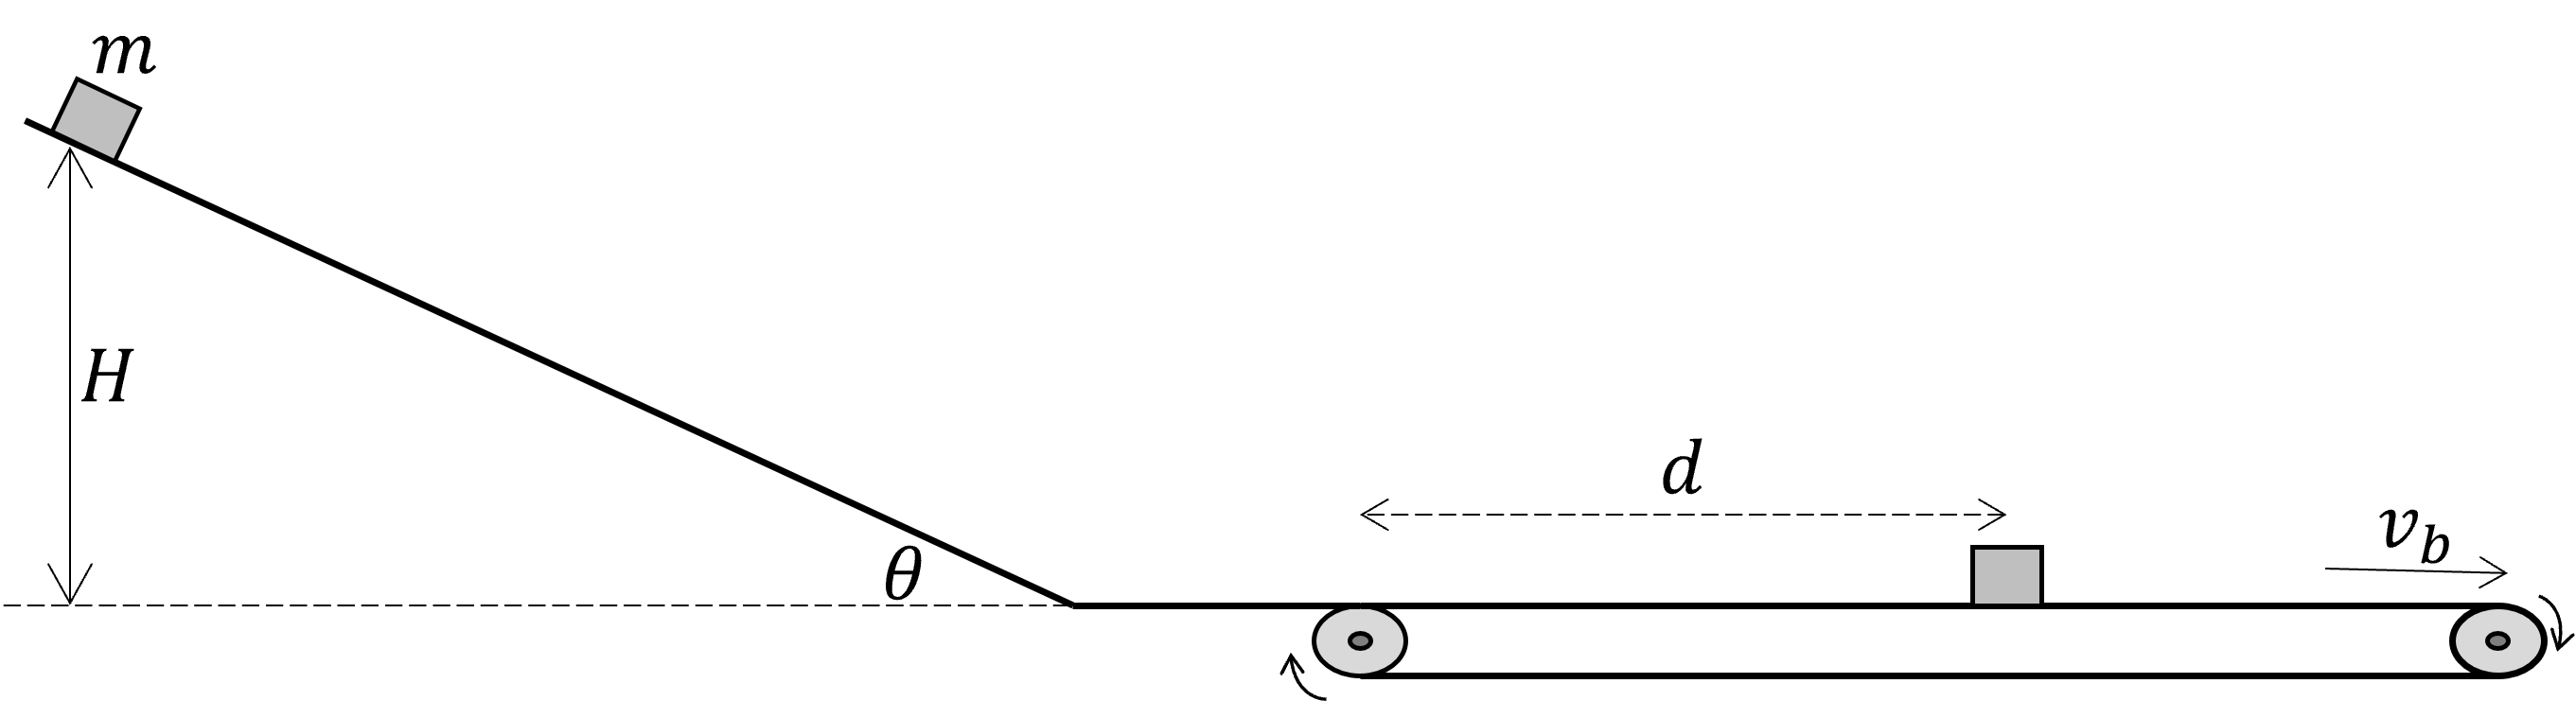
\includegraphics[width=0.8\linewidth]{2023-1/img/TD 3/cinta.png}
\end{figure}



% Para imágenes vectoriales -> el texto tiene que estar en LaTeX
% \begin{figure}[htbp]
%   \centering
%   \svgpath{../Imagenes/ejercicios}  -> .. irse pa'trás 
%   \includesvg{ej5.svg}
% \end{figure}

\end{enumerate}
\end{document}